% ========================================================================
% Supplementary Material
% Companion to the main report
%   "Improving HTR Attention Maps with Register Tokens"
%
% Build:  pdflatex supplementary.tex && bibtex supplementary &&
%         pdflatex supplementary.tex && pdflatex supplementary.tex
% ========================================================================

\documentclass[11pt,a4paper]{article}

\usepackage[utf8]{inputenc}
\usepackage[T1]{fontenc}
\usepackage{lmodern}
\usepackage{amsmath,amssymb,amsfonts}
\usepackage{graphicx}
\usepackage{textcomp}
\usepackage{xcolor}
\usepackage{cite}
\usepackage{booktabs}
\usepackage{array}
\usepackage{multirow}
\usepackage{url}
\usepackage[margin=2.3cm]{geometry}
\usepackage[hidelinks]{hyperref}

\graphicspath{{./figures/}}

\newcommand{\ie}{\textit{i.e.}}
\newcommand{\eg}{\textit{e.g.}}
\newcommand{\etal}{\textit{et al.}}

\title{\textbf{Supplementary Material}\\[0.3em]
\large Improving HTR Attention Maps with Register Tokens:\\
A CTC Vision Transformer for Interpretable Handwritten Text Recognition}

\author{Monika Radhakisan Chavan\\
M.Sc.\ Artificial Intelligence, FAU Erlangen-N\"urnberg\\
Supervisor: Prof.\ Vincent Christlein, Pattern Recognition Lab}

\date{Compiled: \today}

\begin{document}
\maketitle

\begin{abstract}
This document accompanies the main report and collects the material that would clutter the main storyline: per-group training-curve figures (which are cited but not shown in Section~5 of the main report), the run-by-run index of the $63$-experiment matrix, extended attention-quality panels, and detailed extension proposals for future work. It is self-contained; every reference to the main report is prefixed with ``M-'' (e.g.\ M-Sec.~5.3, M-Fig.~5.2). Nothing in this document changes the claims of the main report; it only expands the evidence that supports them and the roadmap they point to.
\end{abstract}

\tableofcontents
\bigskip

% ------------------------------------------------------------------------
\section{Per-Group Training Curves}
\label{supp:curves}

The main report keeps a single training-curve figure (M-Fig.~5.1) that overlays the ViT-RGTS~v2 register sweep on IAM. The five figures in this section show, at the same level of detail, the training curves for the four remaining experiment groups from M-Sec.~4.2: architecture ablations, pretrained-lane fine-tuning, SWA-configuration ablations, READ2016 generalization, and synthetic pretraining. Each figure plots test-CER against epoch for every run in its group, with the best model per group highlighted.

\begin{figure}[h!]
\centering
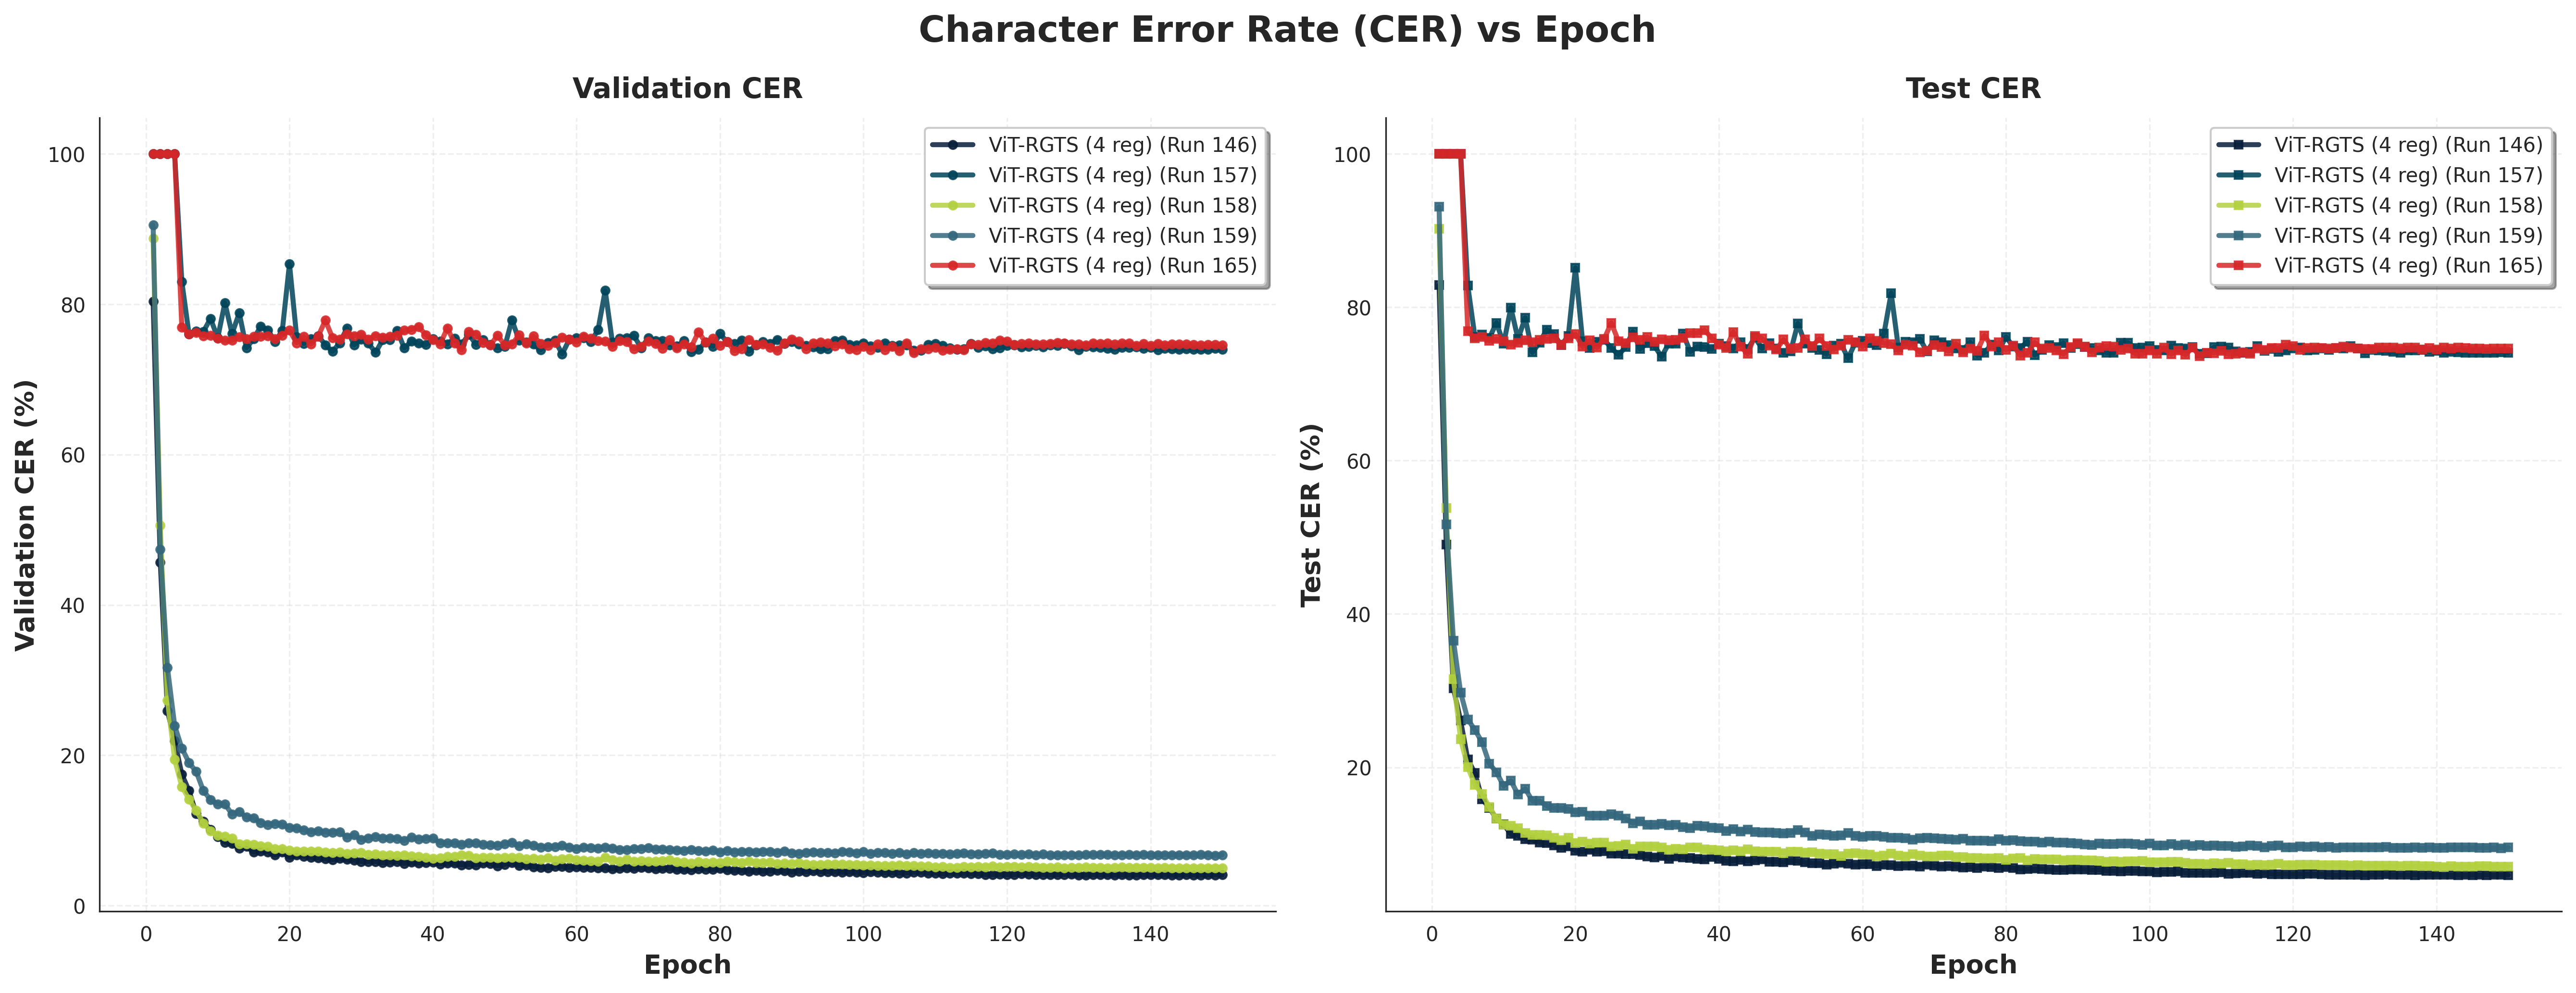
\includegraphics[width=0.95\linewidth]{supp_training_curves_ablations_cer}
\caption{Test-CER convergence for the architecture ablation group (M-Sec.~5.4). The two catastrophically-failing rows (no CNN stem, legacy v1) plateau at ${\sim}73\%$ from epoch~$1$ and are visible as flat lines at the top of the plot; all other ablations converge to the $5$--$10\%$ band by epoch~$50$.}
\label{fig:supp_ablations}
\end{figure}

\begin{figure}[h!]
\centering
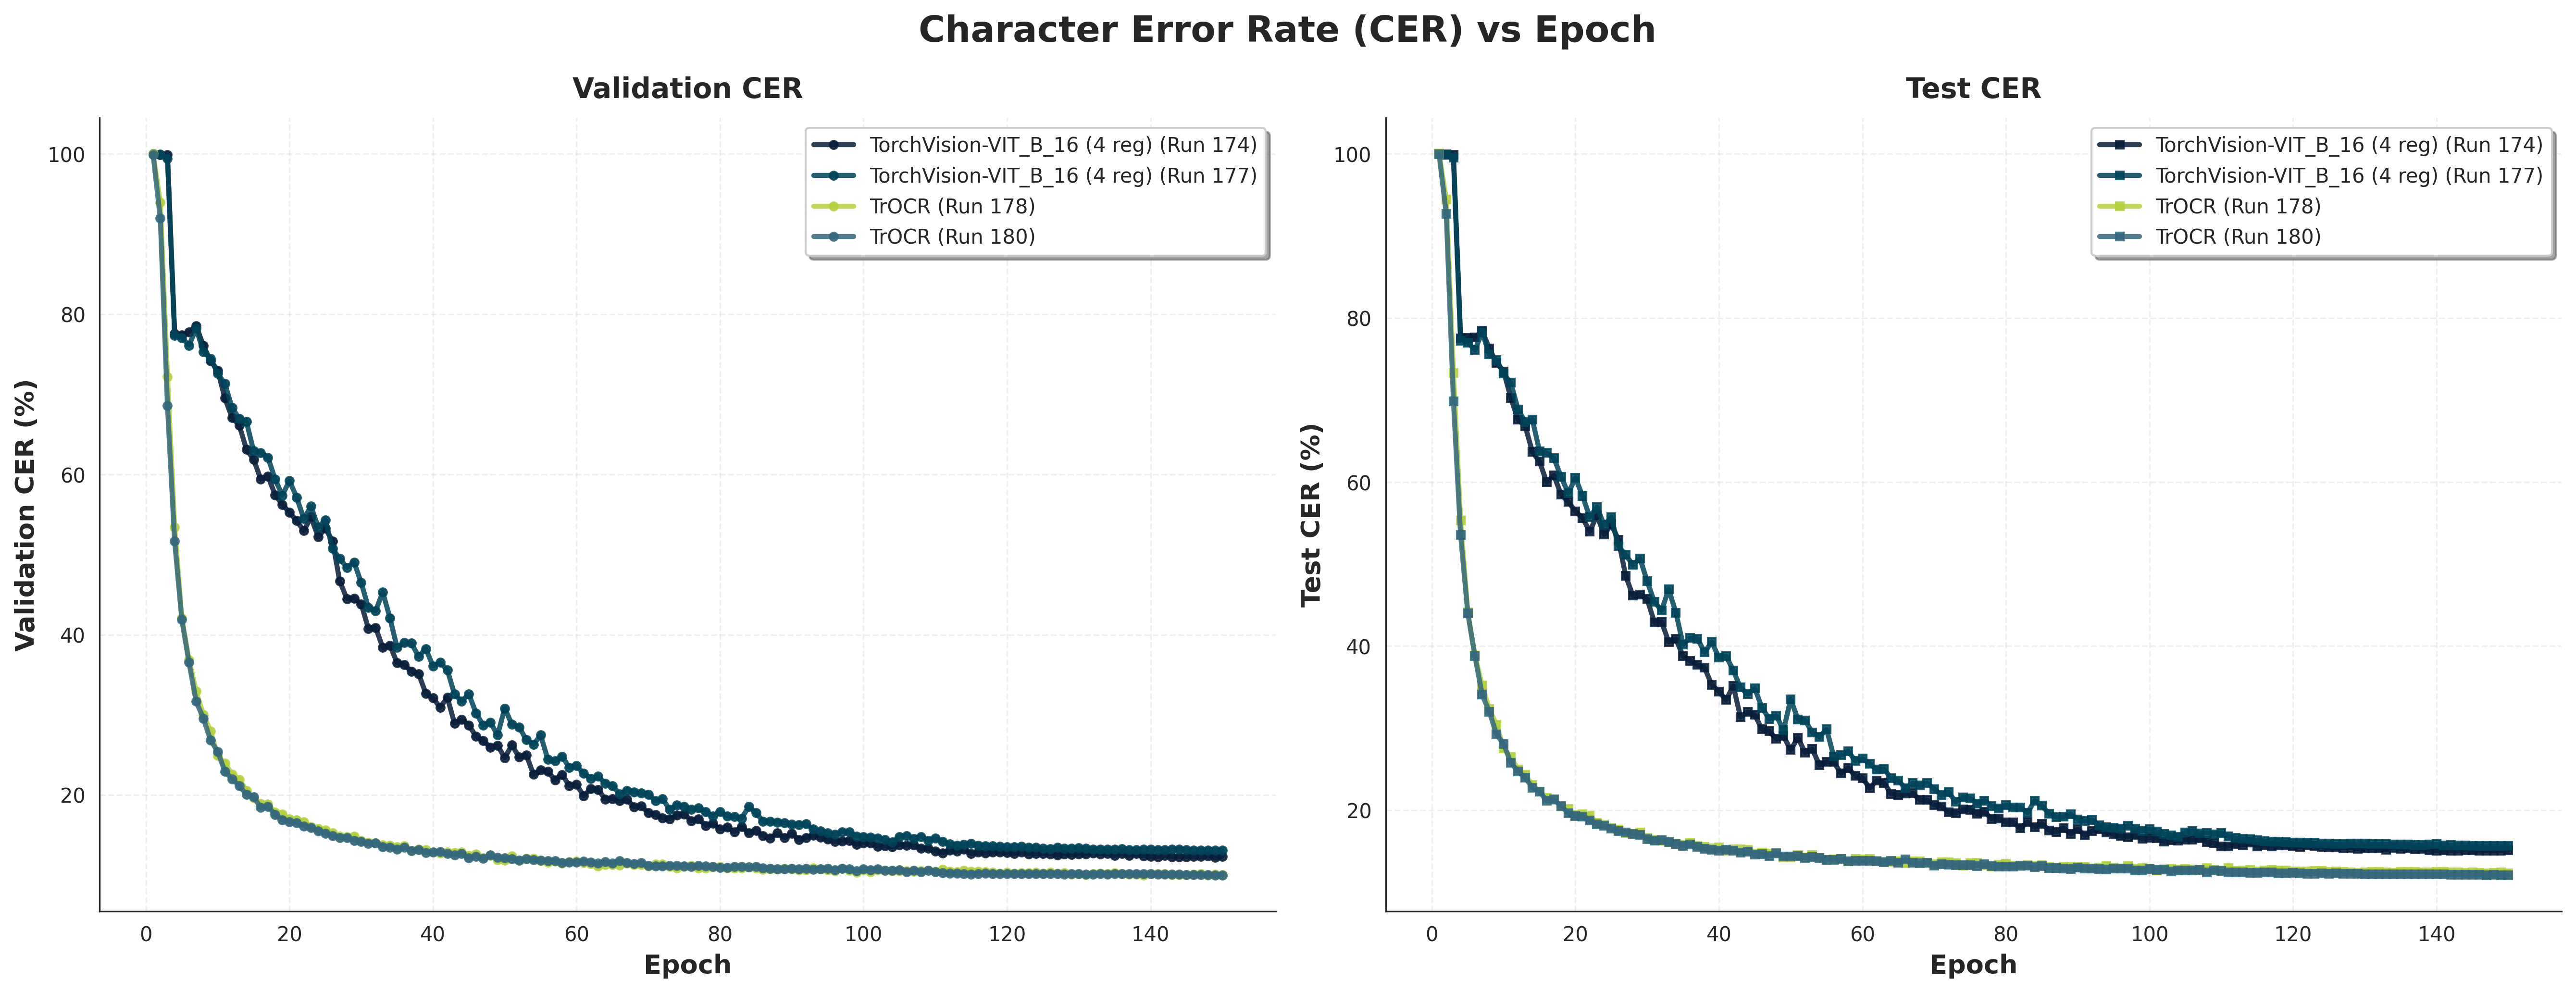
\includegraphics[width=0.95\linewidth]{supp_training_curves_pretrained_cer}
\caption{Test-CER convergence for the pretrained-lane fine-tuning group (M-Sec.~5.5). The naive uniform-LR ViT-B/16 run stays above $70\%$ throughout; two-group LR and LLRD converge cleanly. Note the different y-axis behaviour between the two groups: the naive-run trajectory is not slow convergence but a stuck optimizer.}
\label{fig:supp_pretrained}
\end{figure}

\begin{figure}[h!]
\centering
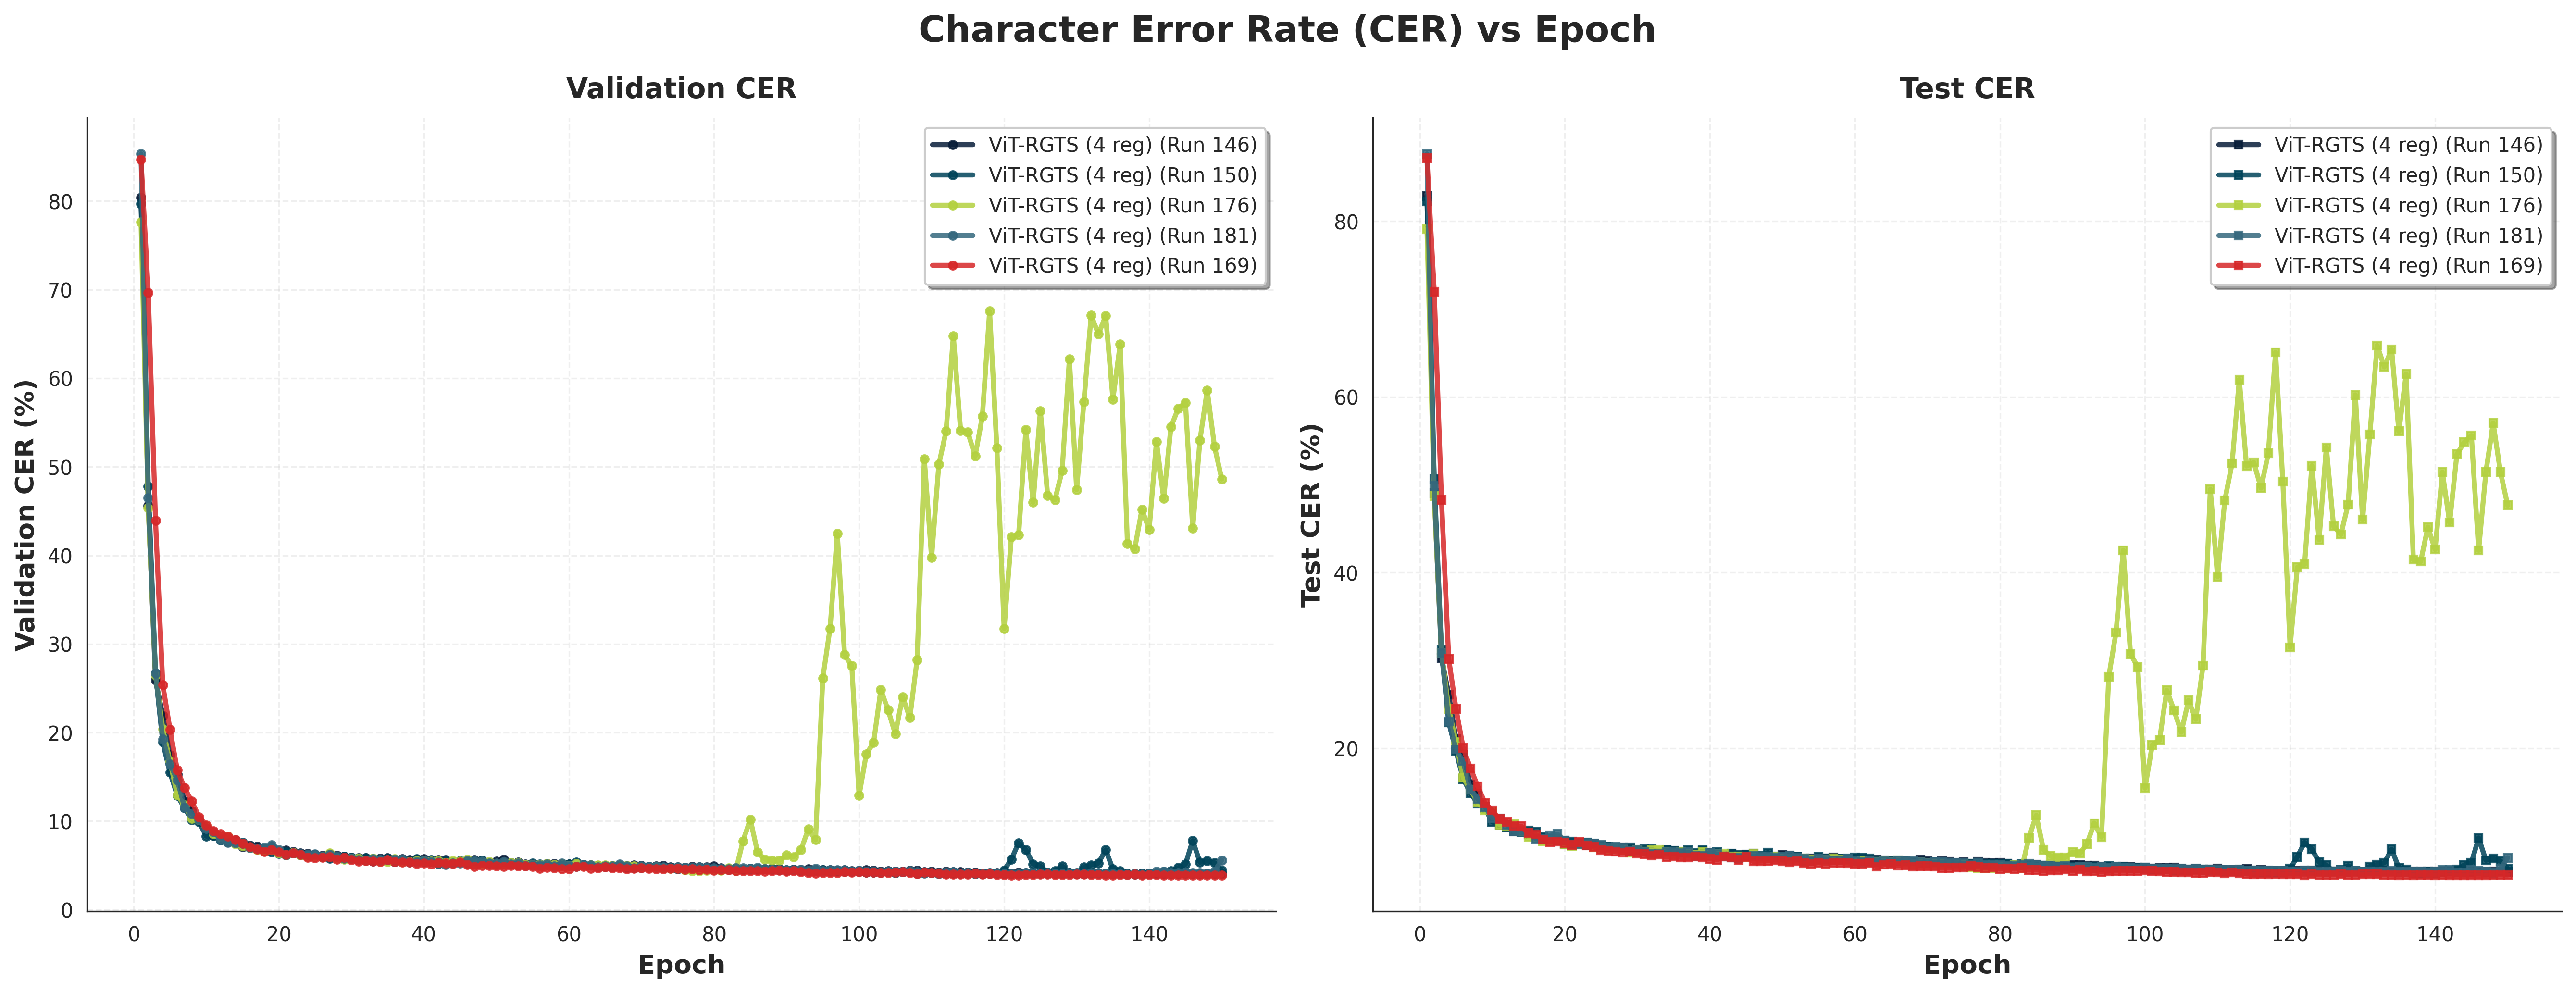
\includegraphics[width=0.95\linewidth]{supp_training_curves_swa_ablation_cer}
\caption{Test-CER convergence for the SWA-configuration ablation (M-Sec.~5.4). SWA-enabled runs show the characteristic ``bump'' at the SWA start epoch as SWALR raises the live-network LR back up; the SWA-averaged model, evaluated separately after BatchNorm recalibration, is not visible in this plot and is reported numerically in the main report (M-Table~5.1).}
\label{fig:supp_swa}
\end{figure}

\begin{figure}[h!]
\centering
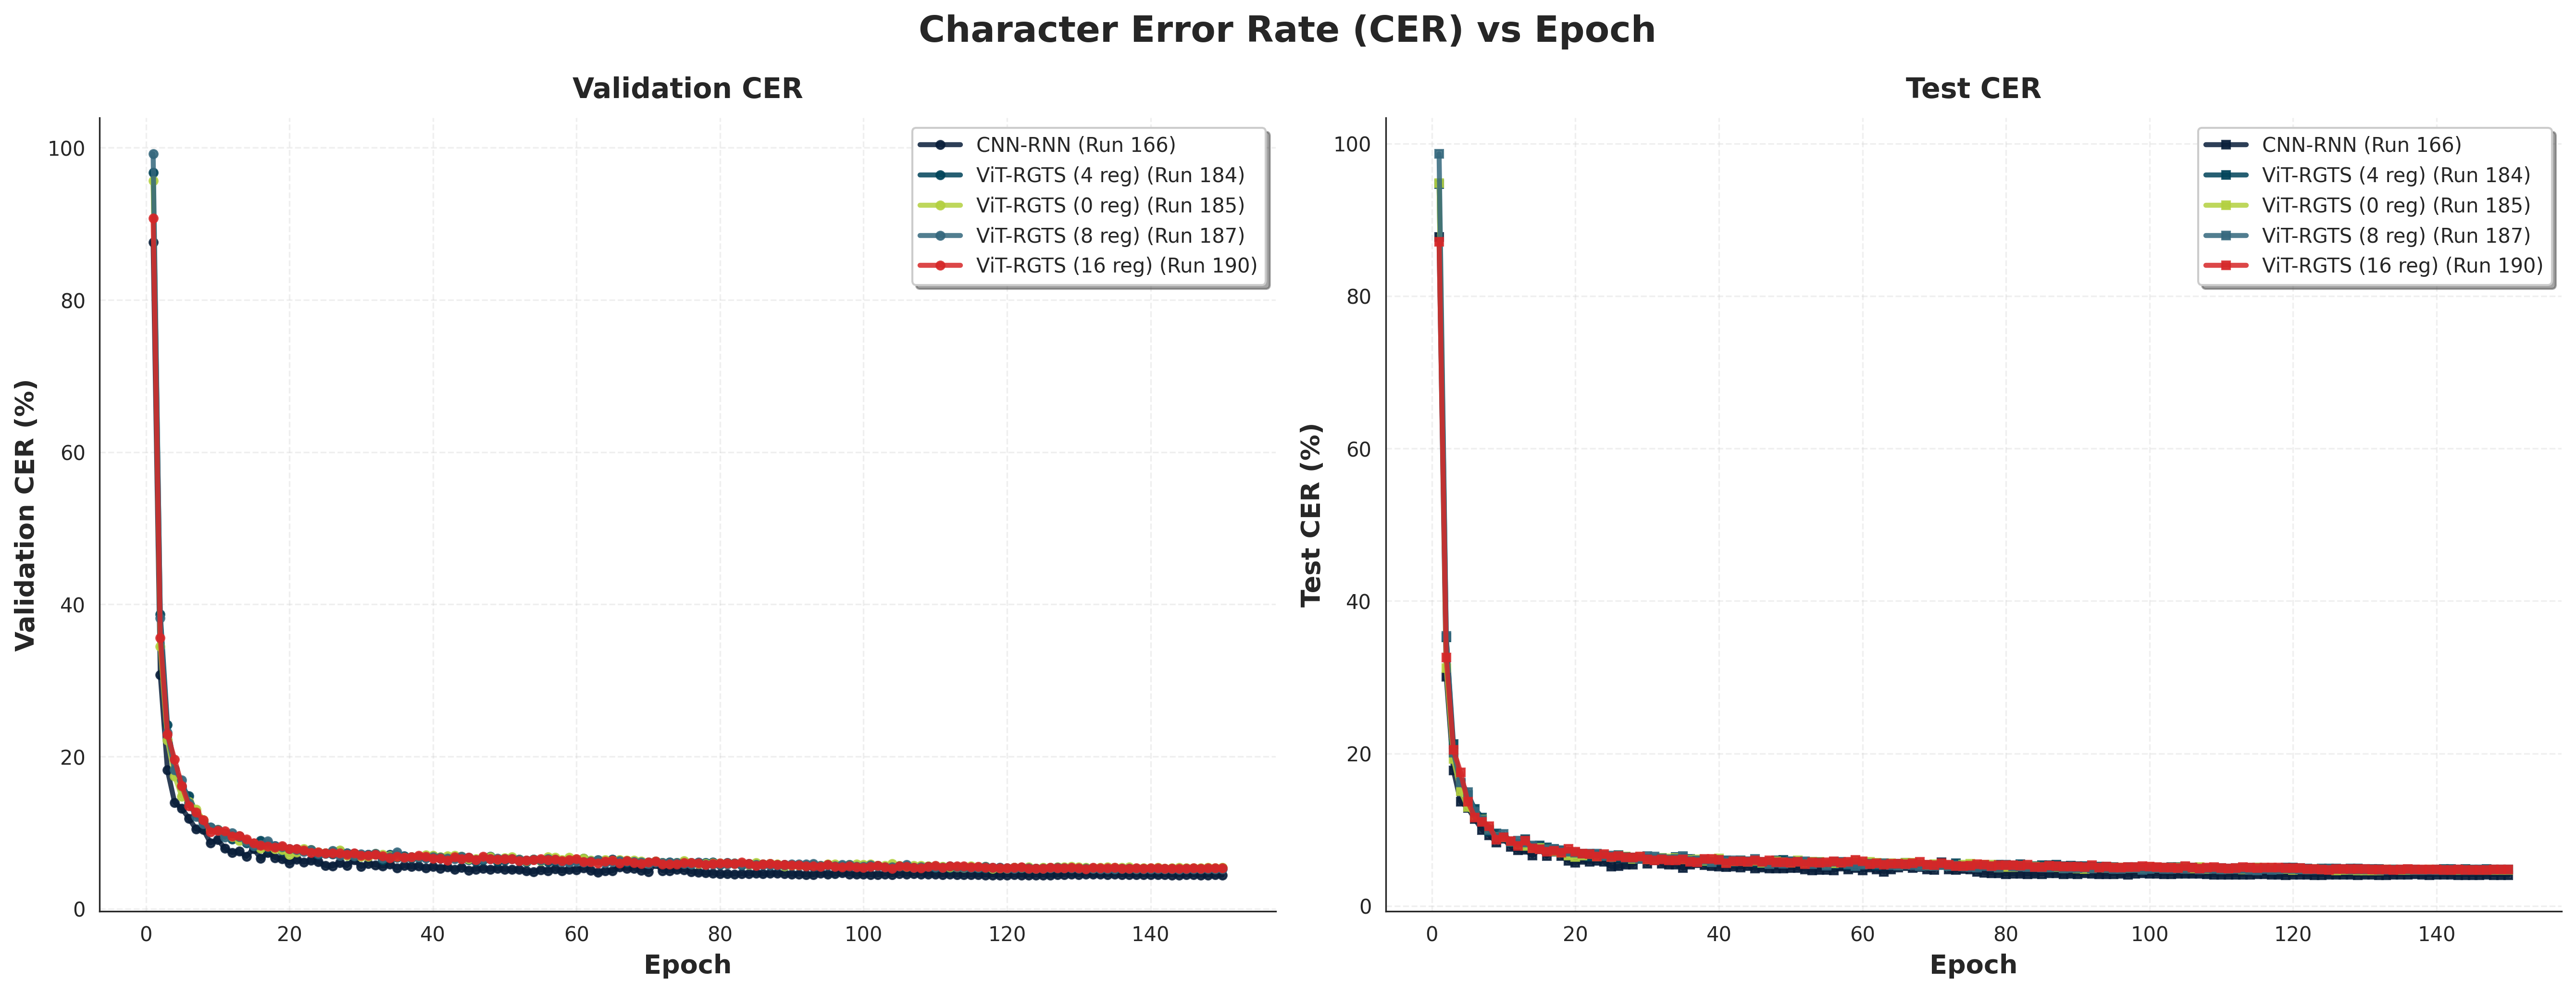
\includegraphics[width=0.95\linewidth]{supp_training_curves_read2016_cer}
\caption{Test-CER convergence for the READ2016 group (M-Sec.~5.6). All ViT-RGTS~v2 register variants converge to essentially the same trajectory, mirroring the IAM behaviour of M-Fig.~5.1.}
\label{fig:supp_read2016}
\end{figure}

\begin{figure}[h!]
\centering
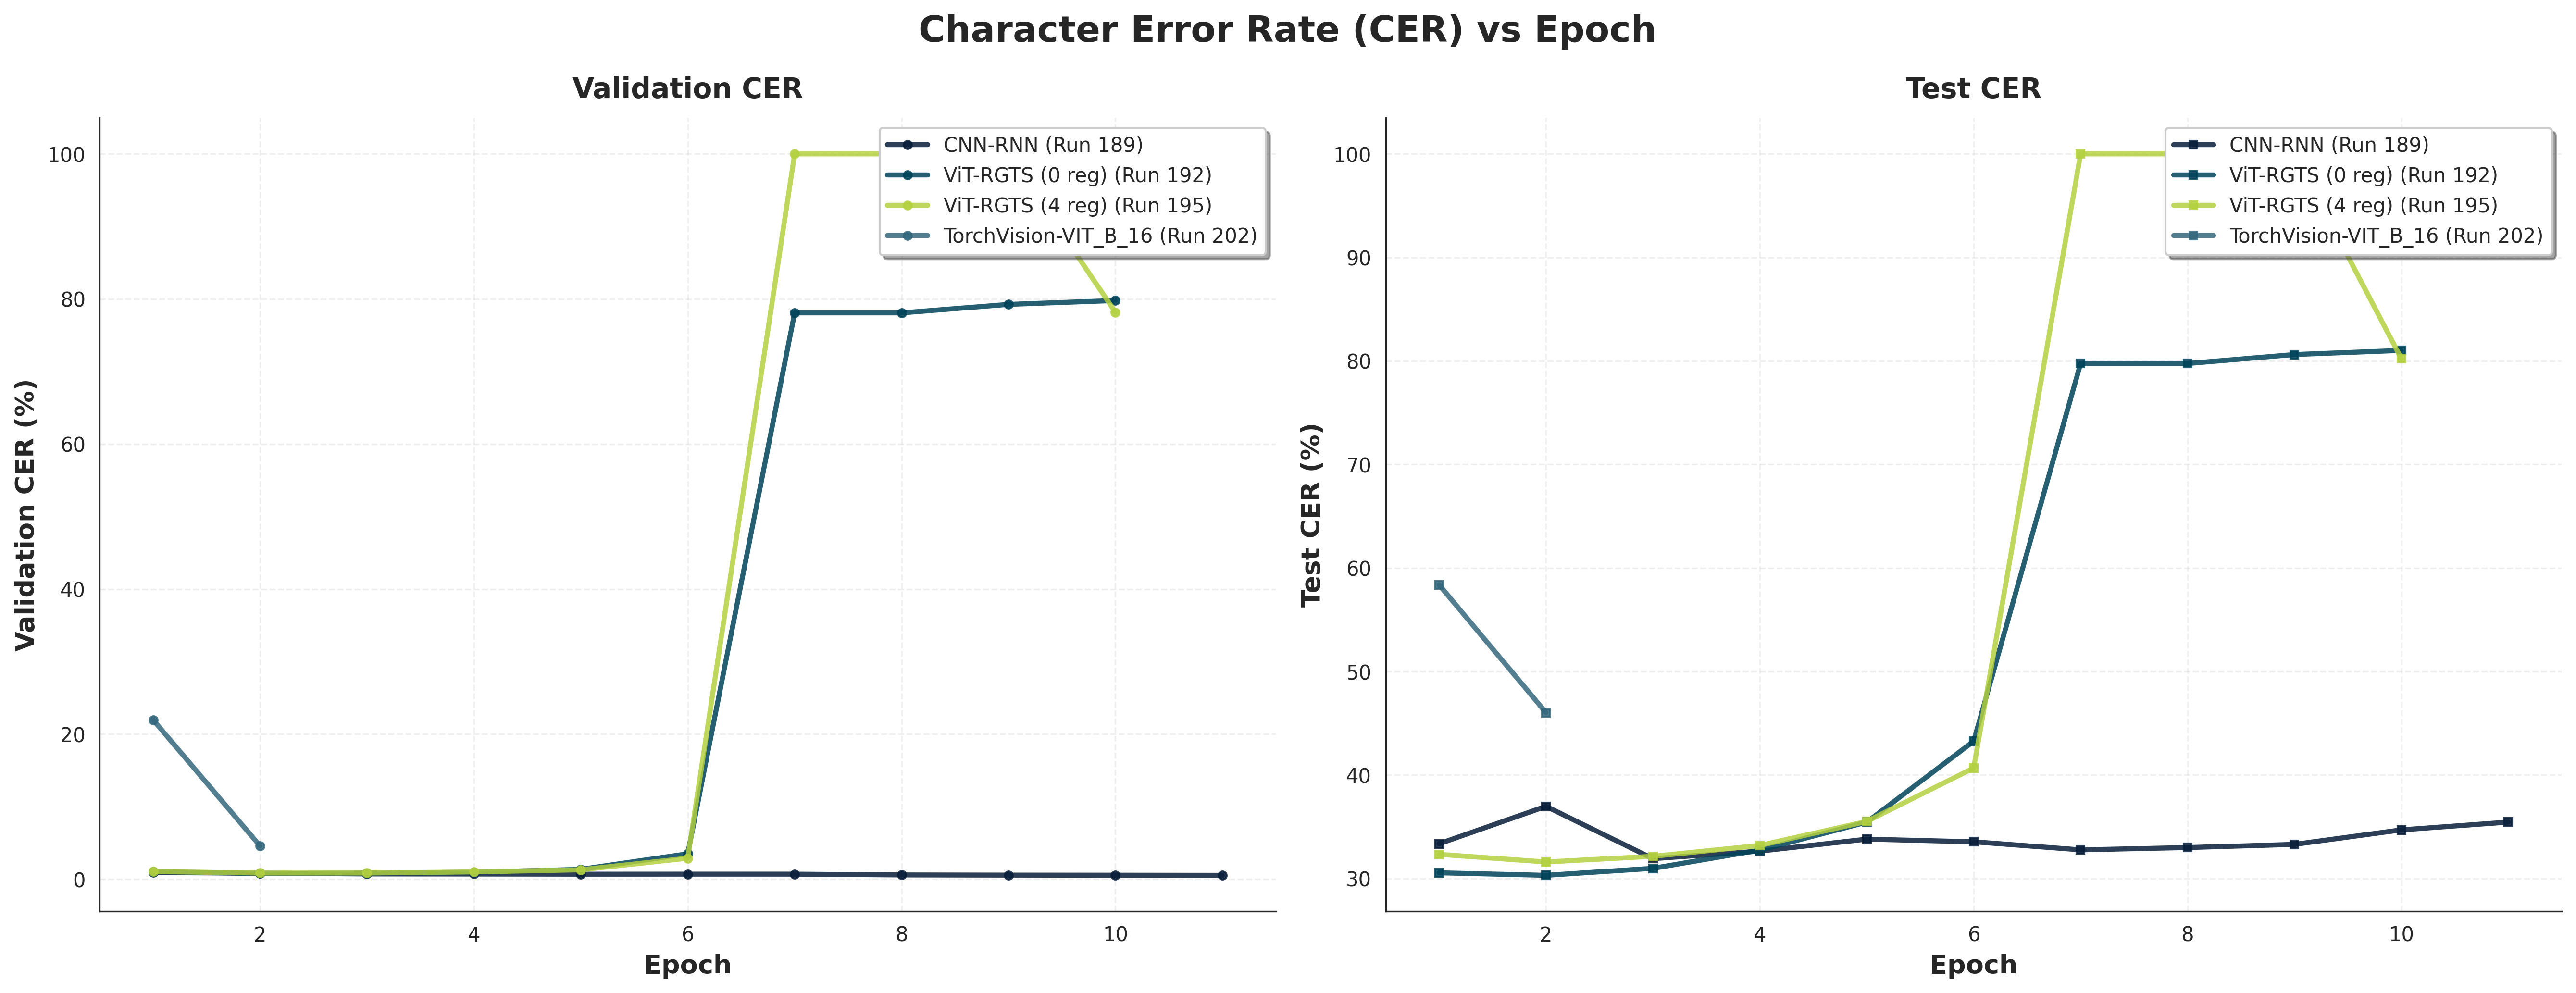
\includegraphics[width=0.95\linewidth]{supp_training_curves_synthetic_cer}
\caption{Test-CER convergence for the synthetic-pretraining group (M-Sec.~5.7). Curves terminate at the $24$-hour SLURM walltime rather than at their intended $15$-epoch budget; the reported CER numbers in the main report are lower bounds on convergence.}
\label{fig:supp_synthetic}
\end{figure}

% ------------------------------------------------------------------------
\clearpage
\section{Run Index}
\label{supp:runs}

Table~\ref{tab:run_index} enumerates all $63$ training runs referenced in the main report, with the configuration file that produced each and the resulting best-validation CER. Runs are stored on disk under \texttt{saved\_models/experiments/run\_N/} with \texttt{config.json}, \texttt{results.csv}, \texttt{training.log}, and (for the register sweep runs) \texttt{attention\_weights/} directories.

\begin{table}[h]
\centering
\small
\caption{Run index for all 63 experiments cited in the main report. Runs marked $\dagger$ were walltime-truncated.}
\label{tab:run_index}
\begin{tabular}{lp{6.5cm}l}
\toprule
Block & Runs & Reference \\
\midrule
Register sweep (IAM) & 143--156, 172 & M-Sec.~5.1, M-Table~5.1 \\
Pretrained lanes (IAM) & 153--155, 173--174, 177--178, 180, 182--183 & M-Sec.~5.5, M-Table~5.4 \\
Architecture ablations & 157--165, 175, 179 & M-Sec.~5.4, M-Table~5.3 \\
Training-strategy ablations & 167--171, 176, 181, 183, 186, 188 & M-Sec.~5.4 \\
READ2016 generalization & 166, 184--185, 187, 190 & M-Sec.~5.6, M-Table~5.5 \\
Synthetic pretraining$^\dagger$ & 189, 191--205 & M-Sec.~5.7 \\
Reproducibility seeds & 146 (seed 42), 170 (seed 123), 171 (seed 456) & M-Sec.~5.8 \\
HTR-VT external comparator & 142 (READ2016) & M-Sec.~5.6 \\
\bottomrule
\end{tabular}
\end{table}

The public reproducibility artifact for this report is the set of $63$ \texttt{run\_N/config.json} files plus the aggregated \texttt{outputs/tables/*.tex} tables cited in the main report. A single \texttt{scripts/postprocessing/aggregate\_results.py} regenerates every table from the raw \texttt{results.csv}/\texttt{training.log} pairs, so any downstream reader can start from the raw run logs and recover the published numbers exactly.

% ------------------------------------------------------------------------
\section{Extended Attention-Quality Analysis}
\label{supp:attn_extra}

The main report reproduces the Nikolaidou~\etal\ Fig.~5 visualization on the single word ``booklet'' (M-Fig.~5.2) and reports the aggregate attention-quality metrics on eight test lines (M-Fig.~5.3). This section fills in two intermediate views.

\subsection{Per-character maps at $R = 0$ vs.\ $R = 4$ for a matched word}

The per-character panels in \texttt{outputs/beyond\_memorization/charIndex\_0/} correspond to the $R = 0$ ViT-RGTS~v2 baseline; the equivalent panels in \texttt{outputs/beyond\_memorization/charIndex\_2/} correspond to the $R = 4$ variant, and \texttt{outputs/beyond\_memorization/noChange/} contains the input-only reference. Reading the two directories side by side confirms qualitatively what M-Fig.~5.3 reports quantitatively: the peak shifts more cleanly with the character index at $R = 4$, and the secondary lobe on unrelated patch columns is smaller. A full pairwise walkthrough of all sixteen words in the fixed test sample is available in \texttt{outputs/beyond\_memorization/comparison\_test/}.

\subsection{Register-absorption trace across layers}

The register-share metric $\alpha_{\mathrm{reg}}^{(\ell)}$ defined in M-Sec.~4.4 grows from ${\sim}0.05$ at $\ell = 1$ to ${\sim}0.18$ at $\ell = 6$ (\ie\ registers absorb an increasing fraction of attention with encoder depth). At $R = 0$ this quantity is zero by definition; at $R = 16$ it saturates at ${\sim}0.35$ regardless of the layer. This layer-wise growth pattern is what a working register mechanism should show, and it is consistent with the pattern Darcet~\etal\ report for classification ViTs. The residual sink pattern noted in the main report therefore does not come from registers being unused; it comes from patch tokens simultaneously being high-norm carriers of the sink information, as explained in M-Sec.~5.3 and M-Sec.~6.1.

% ------------------------------------------------------------------------
\section{Extension Proposals}
\label{supp:extensions}

This section expands the four extensions announced in M-Sec.~7.1 with the specific design decisions each requires.

\subsection{Writer identification via VLAC over ViT-RGTS attention}

The Souibgui~\etal~\cite{souibgui2022vlac} pipeline builds a per-page writer descriptor by aggregating character-indexed local descriptors weighted by the recognizer's per-character attention. The concrete plug-in is:

\begin{enumerate}
    \item Run ViT-RGTS~v2 ($R = 4$) in inference mode and extract, for every recognized character $c$ in every line of every training-set page: the CTC decoding column $t_c$, the patch-token embedding $\mathbf{p}_{t_c} \in \mathbb{R}^{D}$ from the final Transformer layer, and the attention weight vector $\mathbf{a}_c$ over patches from the character's query.
    \item Codebook the patch-token embeddings across the training corpus into $K$ character-prototype clusters (VLAC uses $K$ around the alphabet size).
    \item Assign each character to its nearest prototype and accumulate residual VLAC-style aggregates per prototype into a per-page descriptor.
    \item Evaluate writer-retrieval mAP, top-1, and top-5 on IAM writer-ID splits.
\end{enumerate}

Two design choices differ from the Souibgui~\etal\ original: the descriptor is now attention-weighted rather than character-position-weighted, and the character-detector is the CTC decoder rather than a separate character segmenter. Both simplifications are natural in a ViT-RGTS~v2-based pipeline, and quantifying the writer-ID accuracy is the single most direct test of whether the ``interpretability'' claim of this report translates into a downstream task.

\subsection{CLS-augmented CTC ViT}

The residual sink pattern documented in M-Sec.~5.3(iii) is mechanistically attributed to the absence of a CLS-style aggregate query in a CTC ViT. The extension: add a single CLS token in front of the register block, and supervise it with a light auxiliary loss (\eg\ a writer-classification head at training time, which is unrelated to the CTC objective and does not corrupt the primary decoder). The prediction is that (i) CER stays within the same noise band as the current ViT-RGTS~v2 ($5.5$--$6.0\%$), and (ii) the token-norm asymmetry of M-Fig.~5.3(d) flips, with registers now carrying more norm than patches --- the signature Darcet~\etal\ observe for classification ViTs.

\subsection{Attention-entropy regularizer for CTC}

CTC does not penalize an attention map that ``looks bad'' provided the greedy decoding is correct. A low-weight regularizer on the entropy of the final-layer patch attention would provide the missing gradient signal:
\begin{equation}
\label{eq:aux_entropy}
\mathcal{L}_{\mathrm{total}} = \mathcal{L}_{\mathrm{CTC}} + \beta \cdot \frac{1}{|\mathcal{T}|} \sum_{t \in \mathcal{T}} H(\mathbf{a}_t^{(L)}),
\end{equation}
where $H(\cdot)$ is Shannon entropy and $\mathcal{T}$ is the set of CTC-non-blank query positions. The natural starting range for $\beta$ is $\beta \in [10^{-3}, 10^{-2}]$; larger values would flatten attention entirely and hurt recognition. The regularizer should be evaluated jointly against CER and against the entropy/ordering metrics of M-Sec.~4.4, not against CER alone.

\subsection{Synthetic$\to$IAM curriculum}

The synthetic-pretraining lane in the main report was walltime-truncated. A converged version would:

\begin{enumerate}
    \item Pretrain ViT-RGTS~v2 on the ${\sim}950$K synthetic corpus for a fixed epoch budget --- $50$ epochs is a reasonable target given ${\sim}950$K samples per epoch.
    \item Fine-tune on IAM for $50$ epochs with a decayed learning rate (\eg\ $\eta_{\mathrm{ft}} = 3 \times 10^{-4}$, cosine to $10^{-6}$).
    \item Evaluate on IAM test. The prediction, based on Section~M-5.7 lower-bound behaviour, is that the CER converges to the $4.5$--$5\%$ band, matching or exceeding the from-scratch CNN--RNN baseline.
\end{enumerate}

The purpose is to test whether synthetic-only pretraining, followed by a real-data fine-tune, closes the ViT-vs-CNN--RNN gap without changing the register-attention story. A negative result would indicate that either the synthetic corpus itself needs revision (more writer-style diversity, ink-simulation augmentation) or that ViTs at this scale simply need more real-domain training data.

% ------------------------------------------------------------------------
\section{Reproducibility Appendix}
\label{supp:repro}

All experiments used PyTorch $2.1$ with mixed-precision AMP, on the NHR@FAU cluster's \texttt{rtx3080} partition. Seeds were set as \texttt{seed=42} unless otherwise stated, with \texttt{torch.backends.cudnn.deterministic=True} and \texttt{torch.backends.cudnn.benchmark=False}. The complete environment specification (Python $3.10$, PyTorch $2.1$, package versions) is in \texttt{requirements.txt} in the repository root; the compute-cluster SLURM scripts that produced every run are under \texttt{experiments\_execution/slurm\_modular/}. The M-Sec.~5.8 reproducibility experiment used seeds $\{42, 123, 456\}$ with all other configuration held constant, and its outputs (\texttt{run\_146}, \texttt{run\_170}, \texttt{run\_171}) are directly comparable line-for-line.

\bibliographystyle{plain}
\bibliography{references}

\end{document}
